\documentclass{beamer}
\usepackage[utf8]{inputenc}
\usepackage{tikz} 
\usetikzlibrary{arrows.meta}
\usetheme{Madrid}
\usetikzlibrary{backgrounds}
\usepackage{amssymb}
\title{Vertex Cover Problem}
\usetikzlibrary{arrows,decorations.markings}
\subtitle{Exact and Approximation Algorithm}

\author[Kaowsar and Saha]{Iftekhar Hakim Kaowsar - 1705045\\Apurba Saha - 1705056}


\institute[CSE, BUET]
{
	Department of Computer Science and Engineering\\
	Bangladesh University of Engineering and Technology
}
\date{\today}
\definecolor{amazon}{rgb}{0.0,0.5,0.0}
\newcommand\crossmark[1][]{%
	\tikz[scale=0.4,#1]{
		\fill(0,0)--(0.1,0) .. controls (0.5,0.4) .. (1,0.7)--(0.9,0.7) ..  controls (0.5,0.5) ..(0,0.1) --cycle;
		\fill(1,0.1)--(0.9,0.1) .. controls (0.5,0.3) .. (0,0.7)--(0.1,0.7) .. controls (0.5,0.4) ..(1,0.2) --cycle;
	}%
}

\tikzset{
	invisible/.style={opacity=0.2},
	visible on/.style={alt={#1{}{invisible}}},
	alt/.code args={<#1>#2#3}{%
		\alt<#1>{\pgfkeysalso{#2}}{\pgfkeysalso{#3}} % \pgfkeysalso doesn't change the path
	},
}

\begin{document}
	\frame{\titlepage}
	
	\begin{frame}{Real life scenario}
		What is the minimum number of cameras needed to cover the whole place?
		\begin{figure}[t]
			\centering
			\includegraphics[width=0.75\textwidth]{map.png}
			\caption{Map of BUET,Palashi}
		\end{figure}
	\end{frame}
	
	%Ift starts here
	\section{Problem Definition}
	\begin{frame}{Problem Definition}
		\begin{itemize}
			\item \alert{$Def^n:$} Finding smallest subset of vertices, so that for every edge $(u,v)$ at least one of $u$ and $v$ is in the subset.
			\item Example:
			\newline
			\begin{columns}
				\column{0.2\textwidth}
				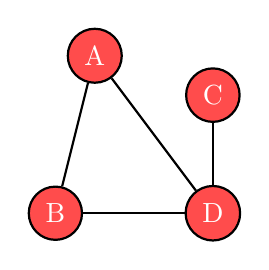
\begin{tikzpicture}[ main/.style = {draw, circle}] 
					\begin{scope}[every node/.style={circle,thick,draw}]
						\node[fill=red!70] (A) at (1.5,3.5) {\textcolor{white}{A}};
						\node[fill=red!70] (B) at (1,1.5) {\textcolor{white}{B}};
						\node[fill=red!70] (C) at (3,3) {\textcolor{white}{C}};
						\node[fill=red!70] (D) at (3,1.5) {\textcolor{white}{D}};
					\end{scope}
					\draw [thick,black] (A) -- (B);
					\draw [thick,black] (B) -- (D);
					\draw [thick,black] (D) -- (A);
					\draw [thick,black] (D) -- (C);
				\end{tikzpicture}
				\column{0.0005\textwidth}
				$\Longrightarrow$
				\column{0.2\textwidth}
				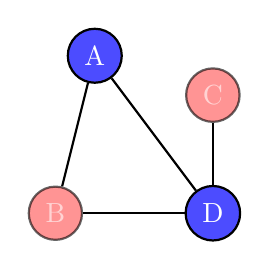
\begin{tikzpicture}[ main/.style = {draw, circle}] 
					\begin{scope}[every node/.style={circle,thick,draw}]
						\node[fill=blue!70] (A) at (1.5,3.5) {\textcolor{white}{A}};
						\node[fill=red!70,opacity=0.6] (B) at (1,1.5) {\textcolor{white}{B}};
						\node[fill=red!70,opacity=0.6] (C) at (3,3) {\textcolor{white}{C}};
						\node[fill=blue!70] (D) at (3,1.5) {\textcolor{white}{D}};
					\end{scope}
					\draw [thick,black] (A) -- (B);
					\draw [thick,black] (B) -- (D);
					\draw [thick,black] (D) -- (A);
					\draw [thick,black] (D) -- (C);
				\end{tikzpicture}
			\end{columns}	
		\end{itemize}
	\end{frame}
	
	
	\section{Exact Algorithm}
	\subsection{Main Idea}
	\begin{frame}{Exact Algorithm}
		Decision version of this problem is whether there is a vertex cover of size at most $K$. \\
		
		Exact algorithm to solve it is quite straight-forward.
		\begin{itemize}
			\item Simply check for all possible subsets of size $K$.
		\end{itemize}
		\alert{Bruteforce!} \\
		\pause 	
		Let's try an example!
	\end{frame}
	
	\subsection{Simulation}
	
	
	\begin{frame}{Exact Algorithm: Simulation}
		\begin{center}
			$K = 3$ \\
		\end{center}
		
		\begin{columns}
			\column{0.5\textwidth}
			
			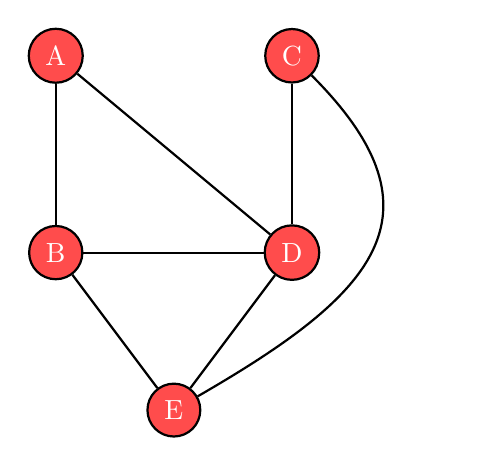
\begin{tikzpicture}[main/.style = {draw, circle}] 
				\begin{scope}[every node/.style={circle,thick,draw}]
					\node[fill=red!70] (A) at (1,4) {\textcolor{white}{A}};
					\node[fill=red!70] (B) at (1,1.5) {\textcolor{white}{B}};
					\node[fill=red!70] (C) at (4,4) {\textcolor{white}{C}};
					\node[fill=red!70] (D) at (4,1.5) {\textcolor{white}{D}};
					\node[fill=red!70] (E) at (2.5,-0.5) {\textcolor{white}{E}};;
				\end{scope}
				\draw [thick,black] (A) -- (B);
				\draw [thick,black] (B) -- (D);
				\draw [thick,black] (A) -- (D);
				\draw [thick,black] (D) -- (C);
				\draw [thick,black] (B) -- (E);
				\draw [thick,black] (E) -- (D);
				\draw [thick,black] (E) to [looseness=1.5,out=30,in=315] (C);
			\end{tikzpicture}
			
			\column{0.5\textwidth}
			
			Subsets of size 3 -- \\
			$\left\{ A, B, C \right\} 
			, \left\{ A, B, D \right\} 
			, \left\{ A, B, E \right\}, \newline
			\left\{ A, C, D \right\} 
			, \left\{ A, C, E \right\}
			, \left\{ A, D, E \right\},  \newline
			\left\{ B, C, D \right\}$
			, ...  									
		\end{columns}
	\end{frame}
	
	\begin{frame}[noframenumbering]{Exact Algorithm: Simulation}
		
		\begin{columns}
			\begin{columns}
				\column{0.5\textwidth}
				
				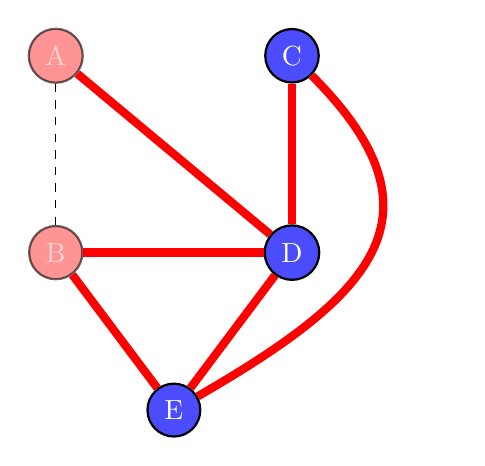
\begin{tikzpicture}[main/.style = {draw, circle}] 
					\begin{scope}[every node/.style={circle,thick,draw}]
						\node[fill=red!70,opacity=0.6] (A) at (1,4) {\textcolor{white}{A}};
						\node[fill=red!70,opacity=0.6] (B) at (1,1.5) {\textcolor{white}{B}};
						\node[fill=blue!70] (C) at (4,4) {\textcolor{white}{C}};
						\node[fill=blue!70] (D) at (4,1.5) {\textcolor{white}{D}};
						\node[fill=blue!70] (E) at (2.5,-0.5) {\textcolor{white}{E}};;
					\end{scope}
					\draw [dashed,black] (A) -- (B);
					\draw [line width=3pt,red] (B) -- (D);
					\draw [line width=3pt,red] (A) -- (D);
					\draw [line width=3pt,red] (D) -- (C);
					\draw [line width=3pt,red] (B) -- (E);
					\draw [line width=3pt,red] (E) -- (D);
					\draw [line width=3pt,red] (E) to [looseness=1.5,out=30,in=315] (C);
				\end{tikzpicture}
				
				\column{0.5\textwidth}
				Check for $\left\{C, D, E\right\}$
				\newline
				\newline
				
				\crossmark[red, scale=1] \alert{Edge $\left(A,B\right)$}	 					
			\end{columns}
		\end{columns}
	\end{frame}
	
	\begin{frame}[noframenumbering]{Exact Algorithm: Simulation}
		
		\begin{columns}
			\begin{columns}
				\column{0.5\textwidth}
				
				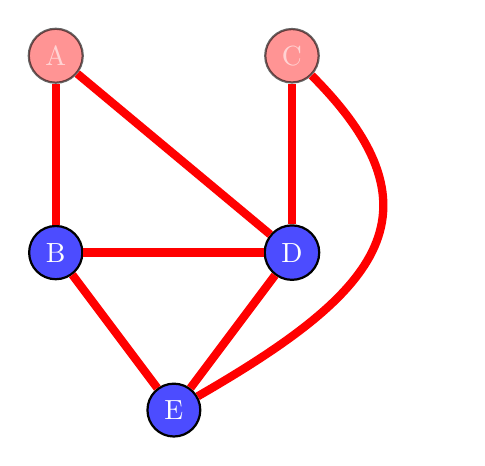
\begin{tikzpicture}[main/.style = {draw, circle}] 
					\begin{scope}[every node/.style={circle,thick,draw}]
						\node[fill=red!70,opacity=0.6] (A) at (1,4) {\textcolor{white}{A}};
						\node[fill=blue!70] (B) at (1,1.5) {\textcolor{white}{B}};
						\node[fill=red!70,opacity=0.6] (C) at (4,4) {\textcolor{white}{C}};
						\node[fill=blue!70] (D) at (4,1.5) {\textcolor{white}{D}};
						\node[fill=blue!70] (E) at (2.5,-0.5) {\textcolor{white}{E}};;
					\end{scope}
					\draw [line width=3pt,red] (A) -- (B);
					\draw [line width=3pt,red] (B) -- (D);
					\draw [line width=3pt,red] (A) -- (D);
					\draw [line width=3pt,red] (D) -- (C);
					\draw [line width=3pt,red] (B) -- (E);
					\draw [line width=3pt,red] (E) -- (D);
					\draw [line width=3pt,red] (E) to [looseness=1.5,out=30,in=315] (C);
				\end{tikzpicture}
				
				\column{0.5\textwidth}
				Check for $\left\{ B, D, E\right\}$
				\newline
				\newline
				
				\textbf{\color{amazon}{\checkmark \space No edge left over}	 		}	\\
				\textbf{\color{amazon}{\checkmark \space Possible vetex cover}	 		}	\\
				We made our decision. \\	
			\end{columns}
		\end{columns}
	\end{frame}
	
	\subsection{Time Complexity}
	\begin{frame}{Time Complexity}
		\begin{itemize}
			\item If Graph has n vertices and m edges, number of possible subsets of size $k$ is $\binom{n}{k}.$ \\
			\item Testing any subset takes $O(m)$ or $O(nk)$ \\
			\item Overall time complexity $O \left( nk\binom{n}{k} \right)$ or $O(k n^{k+1}) $ \\
		\end{itemize}
		\Large{\alert{~~~~~~~~~~~~~~~~~~~~~~~~~~~Too large...}}
	\end{frame}
	
	\section{Parameterized Algorithm}
	\subsection{Main Idea}
	\begin{frame}{Parameterized Algorithm}
		A little different approach.
		\newline
		\newline
		$(u, v)$ is any edge of Graph $G$. \\
		\begin{itemize}
			\item Decision for $(G, k)$ is \textit{yes}, if and only if decision for $(G-u, k-1)$ or $(G-v, k-1)$ is \textit{yes}. \\
			\item If $k=0$, decision is \textit{yes} when there is no edge. \\
		\end{itemize}
		\pause 	
		Let's try an example! \\
	\end{frame}
	
	
	
	\subsection{Simulation}
	\begin{frame}{Parameterized Algorithm: Simulation}
		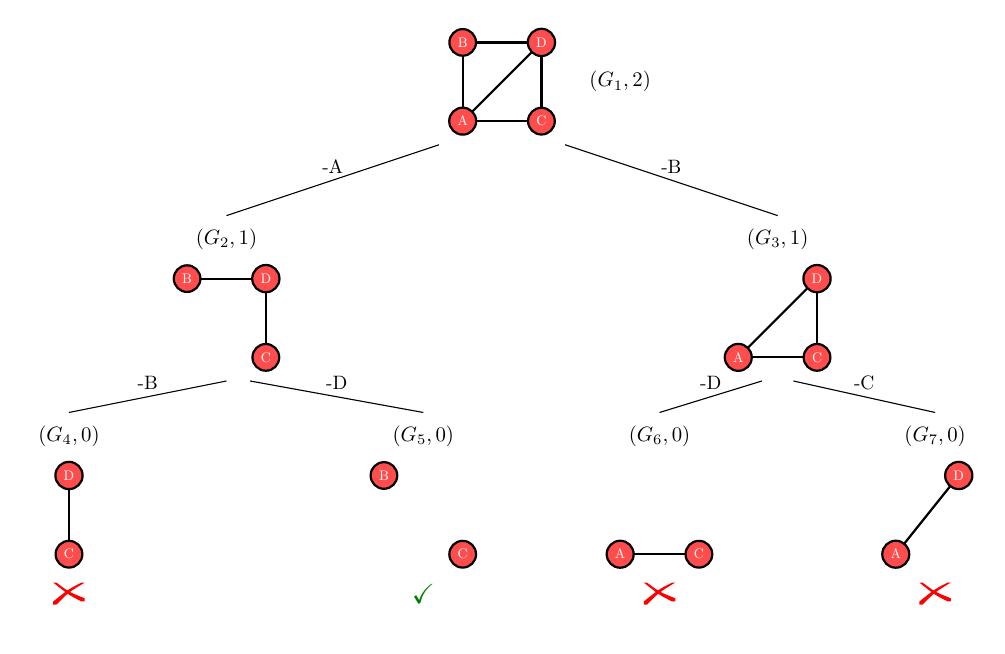
\begin{tikzpicture}[ main/.style = {draw, circle}] 
			\begin{scope}[every node/.style={circle,thick,draw}]
				\node[fill=red!70, scale=0.5] (A) at (0,1) {\textcolor{white}{A}};
				\node[fill=red!70, scale=0.5 ] (B) at (0,2) {\textcolor{white}{B}};
				\node[fill=red!70, scale=0.5] (C) at (1,1) {\textcolor{white}{C}};
				\node[fill=red!70, scale=0.5] (D) at (1,2) {\textcolor{white}{D}};
				\node [draw=none, scale=0.75] at (2,1.5) {$(G_1,2)$};
			\end{scope}
			\draw [thick,black] (A) -- (B);
			\draw [thick,black] (B) -- (D);
			\draw [thick,black] (D) -- (A);
			\draw [thick,black] (D) -- (C);
			\draw [thick,black] (A) -- (C);
			
			\pause
			\draw (-0.3,0.7) -- (-3,-0.2) node[midway,right,above,scale=0.7]{-A};
			\draw (1.3,0.7) -- (4,-0.2)
			node[midway,right,above,scale=0.7]{-B};
			%Rem A from G1, lv 2 -> G2
			\begin{scope}[every node/.style={circle,thick,draw}]
				\node[fill=red!70, scale=0.5 ] (B) at (-3.5,-1) {\textcolor{white}{B}};
				\node[fill=red!70, scale=0.5] (C) at (-2.5,-2) {\textcolor{white}{C}};
				\node[fill=red!70, scale=0.5] (D) at (-2.5,-1) {\textcolor{white}{D}};
				\node [draw=none, scale=0.75] at (-3,-0.5) {$(G_2, 1)$};
			\end{scope}
			\draw [thick,black] (B) -- (D);
			\draw [thick,black] (D) -- (C);
			%Rem B for G1, lv 2 -> G3
			\begin{scope}[every node/.style={circle,thick,draw}]
				\node[fill=red!70, scale=0.5] (A) at (3.5,-2) {\textcolor{white}{A}};
				\node[fill=red!70, scale=0.5] (C) at (4.5,-2) {\textcolor{white}{C}};
				\node[fill=red!70, scale=0.5] (D) at (4.5,-1) {\textcolor{white}{D}};
				\node [draw=none, scale=0.75] at (4,-0.5) {$(G_3, 1)$};
			\end{scope}
			\draw [thick,black] (D) -- (A);
			\draw [thick,black] (D) -- (C);
			\draw [thick,black] (A) -- (C);
			
			\pause
			\draw (-3,-2.3) -- (-5,-2.7) 
			node[midway,right,above,scale=0.7]{-B};
			\draw (-2.7,-2.3) -- (-0.5,-2.7) node[midway,right,above,scale=0.7]{-D};
			%Rem B from G2, lv3 ->G4
			\begin{scope}[every node/.style={circle,thick,draw}]
				\node[fill=red!70, scale=0.5] (C) at (-5,-4.5) {\textcolor{white}{C}};
				\node[fill=red!70, scale=0.5] (D) at (-5,-3.5) {\textcolor{white}{D}};
				\node [draw=none, scale=0.75] at (-5,-3) {$(G_4, 0)$};
				\node [draw=none] at (-5,-5) {\textbf{\color{red}{\crossmark}}};
			\end{scope}
			\draw [thick,black] (D) -- (C);
			
			%Rem D from G3, lv3 -> G5
			\begin{scope}[every node/.style={circle,thick,draw}]
				\node[fill=red!70, scale=0.5 ] (B) at (-1,-3.5) {\textcolor{white}{B}};
				\node[fill=red!70, scale=0.5] (C) at (0,-4.5) {\textcolor{white}{C}};
				\node [draw=none, scale=0.75] at (-0.5,-3) {$(G_5, 0)$};
				\node [draw=none] at (-0.5,-5) {\textbf{\color{amazon}{\checkmark}}};
			\end{scope}
			
			\pause
			\draw (3.8,-2.3) -- (2.5,-2.7) 
			node[midway,right,above,scale=0.7]{-D};
			\draw (4.2,-2.3) -- (6,-2.7) 
			node[midway,right,above,scale=0.7]{-C};
			%Rem C from G3, lv3 -> G6
			\begin{scope}[every node/.style={circle,thick,draw}]
				\node[fill=red!70, scale=0.5] (A) at (2,-4.5) {\textcolor{white}{A}};
				\node[fill=red!70, scale=0.5] (C) at (3,-4.5) {\textcolor{white}{C}};
				\node [draw=none, scale=0.75] at (2.5,-3) {$(G_6, 0)$};
				\node [draw=none] at (2.5,-5) {\textbf{\color{red}{\crossmark}}};
			\end{scope}
			\draw [thick,black] (C) -- (A);
			
			%Rem D from G3, lv3 -> G7
			\begin{scope}[every node/.style={circle,thick,draw}]
				\node[fill=red!70, scale=0.5] (A) at (5.5,-4.5) {\textcolor{white}{A}};
				\node[fill=red!70, scale=0.5] (D) at (6.3,-3.5) {\textcolor{white}{D}};
				\node [draw=none, scale=0.75] at (6,-3) {$(G_7, 0)$};
				\node [draw=none] at (6,-5) {\textbf{\color{red}{\crossmark}}};
			\end{scope}
			\draw [thick,black] (D) -- (A);
		\end{tikzpicture}
	\end{frame}
	\subsection{Complexity}
	\begin{frame}{Parameterized Algorithm: Time Complexity}
		\begin{align*}
			T(n,k) &\leq 2 T(n-1,k-1) + cm \\
			&\leq 2 T(n-1,k-1) + cnk \\
			& ... \hspace{2.5mm} (Iteration) \\
			&= O(2^knk) \\
		\end{align*}
		\pause
		Brute-force algorithm's time complexity was $O(kn^{k+1})$. \\
	\end{frame}
	
	
	
	
	
	
	
	
	
	
	
	
	%	\begin{frame}{Problems with large graphs}
	%		Say, if we have a general graph with 100 nodes and 500 edges and we need to find the minimum vertex cover in this graph.\newline \newline
	%		Can the brute force algorithm that we have seen earlier solve it?
	%		\newline \newline
	%		\onslide<2->\textbf{Well, yes. But how long will it take?}
	%		
	%		\onslide<3->{
	%			\begin{block}{Let's calculate}
	%				Assuming computer can run $10^9$ instructions in one second.\\
	%				The time complexity of the brute force algorithm is $O \left(2 ^ {|V|} \times |E|\right) $.
	%				So, to complete the algorithm it will take
	%				$$ \frac{2^{100}*500}{10^9} = 6.34*10^{23} seconds = 2*10^{16} years!!$$
	%			\end{block}
	%		}
	%	\end{frame}
	\begin{frame}{Approximation algorithm}
		But we cannot use the exact algorithm in large graphs. What is the solution then?\newline\newline
		\onslide<2->{\textbf{Use approximations!}\\}
		\onslide<2->{
			Using approximation algorithms, we can efficiently find a vertex cover that is near-optimal.
		}
	\end{frame}
	\begin{frame}[noframenumbering]{Approximation algorithm}
		Let's see a simple approximation algorithm.
		\begin{block}{Algorithm}
			initialize vertexCover = $\emptyset$\\
			while the graph has at-least one edge:\\
			~~~~pick a random edge $\left(u,v\right)$\\
			~~~~vertexCover = vertexCover $\cup \left\{u,v\right\}$ \\ 
			~~~~remove all incident edges of $u$\\
			~~~~remove all incident edges of $v$\\
		\end{block}
		Time complexity : $O(|V|+|E|)$
	\end{frame}
	\begin{frame}{Approximation algorithm: Simulation}
		Let's consider a graph $G$, which has $7$ vertices and $9$ edges and simulate the algorithm mentioned.\newline
		\begin{columns}
			\column{0.1\textwidth}
			\column{0.5\textwidth}
			
			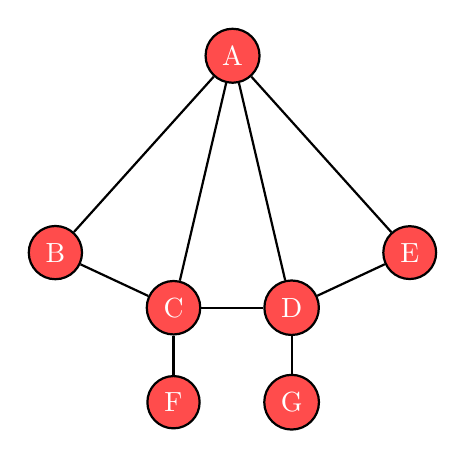
\begin{tikzpicture}[main/.style = {draw, circle}] 
				\begin{scope}[every node/.style={circle,thick,draw}]
					\node[fill=red!70] (A) at (3.25,4) {\textcolor{white}{A}};
					\node[fill=red!70] (B) at (1,1.5) {\textcolor{white}{B}};
					\node[fill=red!70] (C) at (2.5,0.8) {\textcolor{white}{C}};
					\node[fill=red!70] (D) at (4,0.8) {\textcolor{white}{D}};
					\node[fill=red!70] (E) at (5.5,1.5) {\textcolor{white}{E}};
					\node[fill=red!70] (F) at (2.5,-0.4) {\textcolor{white}{F}} ;
					\node[fill=red!70] (G) at (4,-0.4) {\textcolor{white}{G}} ;
				\end{scope}
				\draw [thick,black] (A) -- (B);
				\draw [thick,black] (A) -- (C);
				\draw [thick,black] (A) -- (D);
				\draw [thick,black] (A) -- (E);
				\draw [thick,black] (B) -- (C);
				\draw [thick,black] (C) -- (D);
				\draw [thick,black] (D) -- (E);
				\draw [thick,black] (C) -- (F);
				\draw [thick,black] (D) -- (G);
			\end{tikzpicture}
			\textbf{\newline \newline \text{~~~~~~Vertex cover = $\emptyset$}
			}
			\column{0.4\textwidth}
			The vertices are $\left\{A,B,C,D,E,F,G\right\}$\newline
			The edges are\\
			1. $(A,B)$\\
			2. $(A,C)$\\
			3. $(A,D)$\\
			4. $(A,E)$\\
			5. $(B,C)$\\
			6. $(C,D)$\\
			7. $(D,E)$\\
			8. $(C,F)$\\
			9. $(D,G)$
		\end{columns}
	\end{frame}
	\begin{frame}[noframenumbering]{Approximation algorithm: Simulation}
		
		\begin{columns}
			\column{0.1\textwidth}
			\column{0.5\textwidth}
			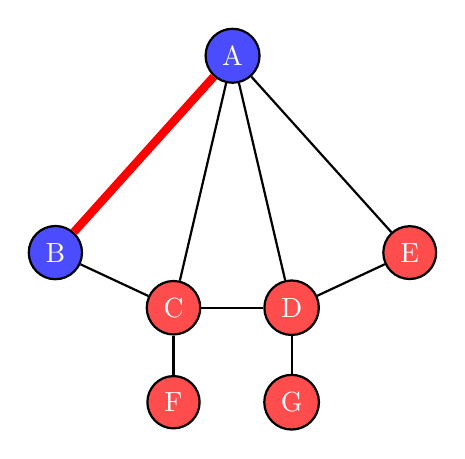
\begin{tikzpicture}[main/.style = {draw, circle}] 
				\begin{scope}[every node/.style={circle,thick,draw}]
					\node[fill=blue!70] (A) at (3.25,4) {\textcolor{white}{A}};
					\node[fill=blue!70] (B) at (1,1.5) {\textcolor{white}{B}};
					\node[fill=red!70] (C) at (2.5,0.8) {\textcolor{white}{C}};
					\node[fill=red!70] (D) at (4,0.8) {\textcolor{white}{D}};
					\node[fill=red!70] (E) at (5.5,1.5) {\textcolor{white}{E}};
					\node[fill=red!70] (F) at (2.5,-0.4) {\textcolor{white}{F}} ;
					\node[fill=red!70] (G) at (4,-0.4) {\textcolor{white}{G}} ;
				\end{scope}
				\draw [line width=3pt,red] (A) -- (B);
				\draw [thick,black] (A) -- (C);
				\draw [thick,black] (A) -- (D);
				\draw [thick,black] (A) -- (E);
				\draw [thick,black] (B) -- (C);
				\draw [thick,black] (C) -- (D);
				\draw [thick,black] (D) -- (E);
				\draw [thick,black] (C) -- (F);
				\draw [thick,black] (D) -- (G);
			\end{tikzpicture}
			\textbf{\newline \newline \text{~~~~~~Vertex cover = $\left\{A,B\right\}$}}
			\column{0.4\textwidth}
			\begin{itemize}
				\item Pick a random edge $\textbf{(A,B)}$ .
				\item Add $\textbf{A}$ and $\textbf{B}$ to the vertex cover set.
			\end{itemize}
		\end{columns}
	\end{frame}
	\begin{frame}[noframenumbering]{Approximation algorithm: Simulation}
		\begin{columns}
			\column{0.1\textwidth}
			\column{0.5\textwidth}
			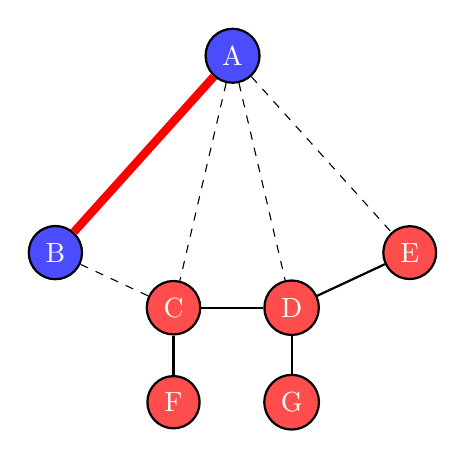
\begin{tikzpicture}[main/.style = {draw, circle}] 
				\begin{scope}[every node/.style={circle,thick,draw}]
					\node[fill=blue!70] (A) at (3.25,4) {\textcolor{white}{A}};
					\node[fill=blue!70] (B) at (1,1.5) {\textcolor{white}{B}};
					\node[fill=red!70] (C) at (2.5,0.8) {\textcolor{white}{C}};
					\node[fill=red!70] (D) at (4,0.8) {\textcolor{white}{D}};
					\node[fill=red!70] (E) at (5.5,1.5) {\textcolor{white}{E}};
					\node[fill=red!70] (F) at (2.5,-0.4) {\textcolor{white}{F}} ;
					\node[fill=red!70] (G) at (4,-0.4) {\textcolor{white}{G}} ;
				\end{scope}
				\draw [line width=3pt,red] (A) -- (B);
				\draw [dashed,black] (A) -- (C);
				\draw [dashed,black] (A) -- (D);
				\draw [dashed,black] (A) -- (E);
				\draw [dashed,black] (B) -- (C);
				\draw [thick,black] (C) -- (D);
				\draw [thick,black] (D) -- (E);
				\draw [thick,black] (C) -- (F);
				\draw [thick,black] (D) -- (G);
			\end{tikzpicture}
			\textbf{\newline \newline \text{~~~~~~Vertex cover = $\left\{A,B\right\}$}}
			\column{0.4\textwidth}
			\begin{itemize}
				\item Remove every edge incident to either $\textbf{A}$ or $\textbf{B}$.
			\end{itemize}
		\end{columns}
	\end{frame}
	\begin{frame}[noframenumbering]{Approximation algorithm: Simulation}
		\begin{columns}
			\column{0.1\textwidth}
			\column{0.5\textwidth}
			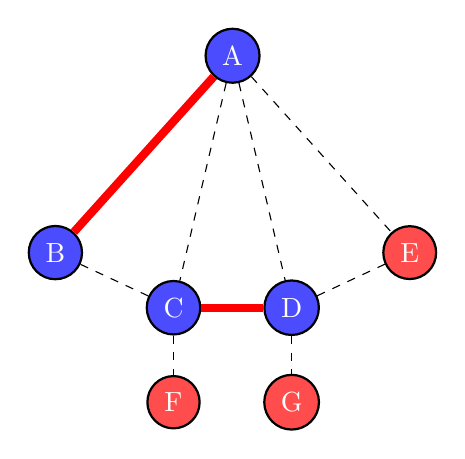
\begin{tikzpicture}[main/.style = {draw, circle}] 
				\begin{scope}[every node/.style={circle,thick,draw}]
					\node[fill=blue!70] (A) at (3.25,4) {\textcolor{white}{A}};
					\node[fill=blue!70] (B) at (1,1.5) {\textcolor{white}{B}};
					\node[fill=blue!70] (C) at (2.5,0.8) {\textcolor{white}{C}};
					\node[fill=blue!70] (D) at (4,0.8) {\textcolor{white}{D}};
					\node[fill=red!70] (E) at (5.5,1.5) {\textcolor{white}{E}};
					\node[fill=red!70] (F) at (2.5,-0.4) {\textcolor{white}{F}} ;
					\node[fill=red!70] (G) at (4,-0.4) {\textcolor{white}{G}} ;
				\end{scope}
				\draw [line width=3pt,red] (A) -- (B);
				\draw [dashed,black] (A) -- (C);
				\draw [dashed,black] (A) -- (D);
				\draw [dashed,black] (A) -- (E);
				\draw [dashed,black] (B) -- (C);
				\draw [line width=3pt,red] (C) -- (D);
				\draw [dashed,black] (D) -- (E);
				\draw [dashed,black] (C) -- (F);
				\draw [dashed,black] (D) -- (G);
			\end{tikzpicture}
			\textbf{\newline \newline \text{~~~~Vertex cover = $\left\{A,B,C,D\right\}$}}
			\column{0.4\textwidth}
			\begin{itemize}
				\item Again pick a random edge $\textbf{(C,D)}$ .
				\item Add $\textbf{C}$ and $\textbf{D}$ to the vertex cover set.
				\item Remove every edge incident to either $\textbf{C}$ or $\textbf{D}$.
			\end{itemize}
			
		\end{columns}
	\end{frame}
	\begin{frame}[noframenumbering]{Approximation algorithm: Simulation}
		\begin{columns}
			\column{0.1\textwidth}
			\column{0.5\textwidth}
			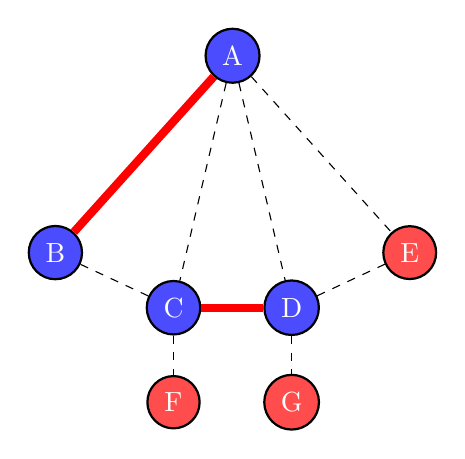
\begin{tikzpicture}[main/.style = {draw, circle}] 
				\begin{scope}[every node/.style={circle,thick,draw}]
					\node[fill=blue!70] (A) at (3.25,4) {\textcolor{white}{A}};
					\node[fill=blue!70] (B) at (1,1.5) {\textcolor{white}{B}};
					\node[fill=blue!70] (C) at (2.5,0.8) {\textcolor{white}{C}};
					\node[fill=blue!70] (D) at (4,0.8) {\textcolor{white}{D}};
					\node[fill=red!70] (E) at (5.5,1.5) {\textcolor{white}{E}};
					\node[fill=red!70] (F) at (2.5,-0.4) {\textcolor{white}{F}} ;
					\node[fill=red!70] (G) at (4,-0.4) {\textcolor{white}{G}} ;
				\end{scope}
				\draw [line width=3pt,red] (A) -- (B);
				\draw [line width=3pt,red] (C) -- (D);
				\draw [dashed,black] (A) -- (C);
				\draw [dashed,black] (A) -- (D);
				\draw [dashed,black] (A) -- (E);
				\draw [dashed,black] (B) -- (C);
				\draw [dashed,black] (D) -- (E);
				\draw [dashed,black] (C) -- (F);
				\draw [dashed,black] (D) -- (G);
			\end{tikzpicture}
			\textbf{\newline \newline \text{~~~~Vertex cover = $\left\{A,B,C,D\right\}$}}
			\column{0.4\textwidth}
			\begin{itemize}
				\item No more edges left to pick. We are done.
				\item We have found a vertex cover of size 4.\newline \newline
			\end{itemize}
			\onslide<2->Is this the minimum cover?
			\onslide<3->\textbf{No! Minimum Vertex Cover is of size 3.}\\$\left\{A,C,D\right\}$
		\end{columns}
	\end{frame}
	\begin{frame}{Result analysis}
		It may seem that our result is quite good.
		But what would have happened if during the second step we had picked the edge $\textbf{(D,E)}$?
		\onslide<2->
		{
			\begin{columns}
				\column{0.1\textwidth}
				\column{0.5\textwidth}
				
				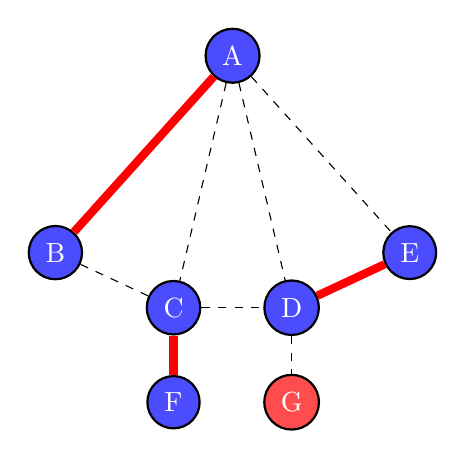
\begin{tikzpicture}[main/.style = {draw, circle}] 
					\begin{scope}[every node/.style={circle,thick,draw}]
						\node[fill=blue!70] (A) at (3.25,4) {\textcolor{white}{A}};
						\node[fill=blue!70] (B) at (1,1.5) {\textcolor{white}{B}};
						\node[fill=blue!70] (C) at (2.5,0.8) {\textcolor{white}{C}};
						\node[fill=blue!70] (D) at (4,0.8) {\textcolor{white}{D}};
						\node[fill=blue!70] (E) at (5.5,1.5) {\textcolor{white}{E}};
						\node[fill=blue!70] (F) at (2.5,-0.4) {\textcolor{white}{F}} ;
						\node[fill=red!70] (G) at (4,-0.4) {\textcolor{white}{G}} ;
					\end{scope}
					\draw [line width=3pt,red] (A) -- (B);
					\draw [dashed,black] (A) -- (C);
					\draw [dashed,black] (A) -- (D);
					\draw [dashed,black] (A) -- (E);
					\draw [dashed,black] (B) -- (C);
					\draw [dashed,black] (C) -- (D);
					\draw [line width=3pt,red] (D) -- (E);
					\draw [line width=3pt,red] (C) -- (F);
					\draw [dashed,black] (D) -- (G);
				\end{tikzpicture}
				\textbf{\newline \newline \text{~~~Vertex cover = $\left\{A,B,C,D,E,F\right\}$}}
				\column{0.4\textwidth}
				This time we get a vertex cover of size $6$ which is  twice the size
				of an optimal vertex cover!!
			\end{columns}
		}
		
	\end{frame}
	\begin{frame}{Result analysis}
		Can it get any worse?\newline\newline
		\onslide<2->
		\textbf{No! The vertex cover returned by APPROXIMATE VERTEX COVER is at most twice the size of an optimal vertex cover. We can also prove that.\\}
	\end{frame}
	\begin{frame}{Proof}
		\begin{block}{Observations}
			\begin{itemize}
				\item In the set of edges that we picked, no two share an endpoint.
				\item If the algorithm picked $k$ edges, the vertex cover found has size $2k$.	
			\end{itemize}
		\end{block}
		From these observations, any vertex cover must have size at least $k$ since it needs to have at least one endpoint of each of these edges, and
		since these edges don’t touch, there are $k$ different vertices. So the algorithm is a factor $2$ approximation.
	\end{frame}
	
	\begin{frame}{Factor 1.99}
		As we have achieved a factor of 2, is it possible to efficiently achieve a factor $1.99$?\newline\newline
		\onslide<2->
		\textbf{Unfortunately, nobody knows if it is possible to efficiently achieve a factor 1.99.\\}
	\end{frame}
	\begin{frame}{}
		\centering \Huge
		\emph{Thank You}
	\end{frame}
	
	
\end{document}